\documentclass[11pt,a4paper]{report}

\usepackage[top=1.5in,bottom=1.5in,left=1in,right=1in]{geometry}
\usepackage{pdflscape}
\usepackage{enumitem}
\usepackage{graphicx}
\usepackage[nottoc]{tocbibind}
\usepackage[square,comma,numbers]{natbib}
\bibliographystyle{IEEEtranS}

\begin{document}
\title{{\normalsize G52GRP Interim Report}\\EduCraft\\\textit{Minecraft as a Collaborative Learning Tool}}
\author{Group \texttt{gp13-pxb1}:\\
            Tosin Afolabi (\texttt{ooa02u})\\
            Janos Bana (\texttt{jxb12u})\\
            Eze Benson (\texttt{exb02u})\\
            Ali Kerr (\texttt{axk02u})\\
            Ian Knight (\texttt{iak12u})\\
            Ying Wang (\texttt{yxw03u})
            }
\maketitle

\tableofcontents

\chapter{Introduction and Background}
The EduCraft project is concerned with developing a series of
extensions\footnote{These are commonly called `mods'. Throughout the report, 
we will refer to our product as `the mod'.} for the popular computer game
Minecraft, aimed at promoting collaborative learning in primary schools,
particularly with reference to numeracy education. In this first section, some
of the advantages of collaborative learning are explored in contrast to
conventional teaching methods, and the game of Minecraft is introduced in the
context of education.

\section{Collaborative learning}
\begin{quote}
``Group interaction allows students to negotiate meanings, to express
themselves in the language of the subject and to establish a more intimate
and dialectical contact with academic and teaching staff than formal
methods permit.'' \cite[p.~1]{jacques00}
\end{quote}
Group work has long been recognised as a key component in any form of
successful education---it enables students to become more involved in their
own work, and to engage with it in a different manner from what is normally
seen in classroms. Johnson and Johnson observe that ``The human species seems
to have a \textit{cooperation imperative}'', and that cooperation plays
a central role in most areas of life \cite[p.~12]{johnson94}.

Collaborative or cooperative learning is contrasted with two other `goal
structures': competitive learning, and individualistic learning. Competitive
learning consists of activities which set the students tasks which some
are expected to `win', by getting the highest score or completing the activity
in the shortest time, for example. Individualistic learning is learning where
there is no interaction between students at all---no comparisons are made,
and students are solely concerned with working by themselves.

Johnson and Johnson argue that each of these goal structures has a role
to play in education, but that each is suitable for different
purposes \cite{johnson94}.  Collaborative learning, specifically, is to
be used in situations where the material being taught is especially
complex or conceptual. This makes it ideal for use in maths lessons:
Yackel, \textit{et al.} describe the benefits of group work in teaching maths
to second-grade\footnote{Roughly equivalent to year 5 (ages 7--8) in the UK}
students in the US \cite{yackel91}.

\section{Minecraft}
\begin{quote}
``Minecraft is a game about breaking and placing blocks. At first, people
built structures to protect against nocturnal monsters, but as the game grew
players worked together to create wonderful, imaginative things.''
\cite{website:minecraft}
\end{quote}

Minecraft was initially developed in 2009, as a game where players could
explore a randomly-generated world and place blocks to build structures. From
the outset, Minecraft was not designed as a game that could be `won'---in
game industry terms, it was intended to be a `sandbox' game where players set
their own goals.

There have been a number of articles written exploring the potential use of
Minecraft in supporting education \cite{brand13}, \cite{short12}. Habgood has
already established the usefulness of computer games in general in education
\cite{habgood07}; the question is whether Minecraft can be used in the ways
that he suggests. This is what EduCraft seeks to establish, at least tentatively.

The official Minecraft Wiki has its own page dedicated to describing possible ways
of using Minecraft in education \cite{website:mcwiki}, and suggests using the
game's in-built system of building items:
\begin{quote}
    ``The crafting system can help in teaching basic math (e.g. I need 3 Sugar 
    Cane for Paper), which transitions to multiplication (I need 3 Paper and 1 
    Leather for a Book, and 3 Books for a Bookshelf, so I need 9 Paper and 3 Leather 
    all together) and division (When I create Paper I get 3 at once, so 9/3 = 
    3 times per Bookshelf I'll have to create Paper).''
\end{quote}

We intend to build something more overtly mathematical than this basic concept,
and the remainder of the report describes the requirements that have been set
for the project, along with a record of our initial design and prototypes.
\chapter{Requirements Specification}

\section{Functional requirements}
\begin{enumerate}

	\item The game must cater for users who are currently at level 2 of keystage 2 mathematics.
	\begin{enumerate}[label={1.\arabic*},nolistsep,leftmargin=*]
		\item There must be a puzzle in the game which challenges the users knowledge of subtraction facts up to 10.
		\item There must be a puzzle in the game which challenges the users knowledge of number ordering from 0 - 100.
		\item There must be a puzzle in the game which challenges the users knowledge of number sequencing. This must include odd and even numbers.
	\end{enumerate}

	\item The game must cater for users who are currently at level 3 of keystage 2 mathematics.
	\begin{enumerate}[label={2.\arabic*},nolistsep,leftmargin=*]
		\item There must be a puzzle in the game which challenges the users knowledge of the 2,3,4,5 and 10 times table.
		\item There must be a puzzle which forces a user to use multiplication or division to solve it. The multiplication or division must only be used with whole numbers. When choosing numbers for division numbers with remainders are to be included.	
		\item The game should include puzzles which involves breaking entities into simple fractions.
		\item Within the game there should be puzzles which require users to equate simple fractions.
	\end{enumerate}
	
		\item The game must cater for users who are currently at level 4 of keystage 2 mathematics.
		\begin{enumerate}[label={3.\arabic*},nolistsep,leftmargin=*]
			\item Puzzles must exist within the game which can only be solved using division by 10 or 100. The entities being divided must be whole numbers.
			\item A puzzle must exist which tests users upon their knowledge of multiplication facts up to 10x10. This puzzle should then go on to test whether the user can quickly derive correct divison facts.
			\item Within the game there should be a puzzle which involves adding and subtracting entities which represent decimal numbers to 2 decimal places.
			\item A puzzle should exist which forces the user to order decimal numbers. These decimal numbers can be up to three decimal places in length.
		\end{enumerate}
		
	\item Levels in the game must be constructed in such a way that each user contributes to a problem before all the users can progress. A user must contribute within the game physically.
	\item The game must not be single player and should allow players in groups of 3-4 to play together.
	\item The players should be able connect to dedicated servers to play the game.
	
	\item The mod must implement coins as one of the visual representations of numbers.
	
	\item The mod must have custom weapons which can be used to defeat zombies.
	
	\item Coins and other visual representations of numbers must be collected by defeating zombies.
	
	\item Zombies must not drop numbers or coins if the user does not defeat them using the specific mathematical weapon.
	
	\item Zombies must have a number above their head clearly visible to the player indicating what number they drop upon being defeated.
	
	\item Zombies should drop a number or coins equal to the number stated above the zombie's head.
	
	\item Players must be able to craft all mathematical operators using items collected throughout the level. (Mathematical operators being +,-,*,/) 
	
	\item Each mathematical operator must be represented visually in a way which is commonly understood by people of the specified age group.
	
	\item Puzzles must be solved in chambers as well as open world spaces.
	
	\item Players should not be allowed to progress until the puzzle they are currently on is completed.
	
	\item Mathematical operators must be usable objects and not weapons.
	
	\item Mathematical operators will be crafted using items which have been ascertained through resource collecting, where resource collecting is the action of getting items in any way but defeating zombies.
	
	\item Equations must be able to be crafted using mathematical operators and numbers collected from defeated zombies.
		
\end{enumerate}

\section{Non-functional requirements}
\begin{enumerate}
	\item The game must be implemented in Minecraft through a mod.
	\item The mod should work on Minecraft version 1.6.4.
	\item The mod must work on the windows operating system.
	\item The mod must work on a machine which has the minimum requirements of Minecraft or better.
	\item The game should abide by the ethics code in place within the education system for those between the ages of 8 and 11.
\end{enumerate}


\chapter{Design and Implementation}

\section{Overview}
A discussion of the design of the system, and key factors that 
influenced our design. We should talk about the requirement to 
develop using Java, and the decision to use the MinecraftForge API.

\section{Using Java}
Minecraft is a game written in the Java language, and so it is 
only logical that when we mod the game it is required that we use 
Java. This links in with the API we use, which is also dependent 
on Java and specifically is made with support for Eclipse (in 
terms for example of online tutorials for setting up and coding 
in the Eclipse JDK environment). 

\section{Decision to use MinecraftForge API}
Before creating our mod we had to choose the method for modding 
the game. Our final choice was to use the MinecraftForge API, which 
is a mod/application layer for Minecraft which lets us create and 
run Minecraft mods. The decision to use MinecraftForge API was 
because of its versatility and usefulness. Furthermore, we decided 
to use MinecraftForge over other alternatives because, while other 
tools like ModLoader may have been arguably easier to use, MinecraftForge 
is much more suited for our purposes – namely, creating a more complex 
mod. This is because MinecraftForge has a lot more possibilities, whereas 
with ModLoader there is more limited scope for creating complex Minecraft 
mods. Aside from ModLoader and MinecraftForge, there wasn’t much else 
choice; these two mod tools are the most popular by far in the Minecraft 
community.  

\section{Discussion of the design of the system}
Because of the very nature of MinecraftForge and our design, 
all modifications are done by creating new classes – we are 
creating a mod that adds and extends from Minecraft, we are 
not creating a core mod. Because of this we have our mod in 
a new package: package org.educraft, which can be implemented 
by MinecraftForge and run in Minecraft. 

Our system design has proxy classes, which at the moment aren’t used 
for much but will be used later (when our mod is more developed) for 
purposes such as rendering entities in the Minecraft world (e.g. monsters, items). 
In the current dummy mod we have produced, we have a base class (DummyMod.java), 
which is the first class that MinecraftForge loads. The base class uses other 
classes such as DummyCoin, DummyAttackHandler etc. These separate classes 
control specific individual elements of the mod. For example, DummyCoin extends 
the item class, and is a custom item that we have created for use in our mod. 
Likewise, we use similar tactics in other classes, such as a ‘maths wand’ 
which extends the Minecraft Sword item, and has unique interactions with other 
aspects of the mod such as our dummy zombie. 

In its current state the mod is obviously fairly basic, but we have the 
foundations for an organised system design which can and will be the basis 
for a sophisticated and elegant mod. A key reason for this system design 
is that it follows the standard format of a MinecraftForge mod, meaning it 
is easy to understand, and is well organised. 

Examples of/ tutorials for MinecraftForge mods informed our decision to 
create our mod following this system design; examples can be found on the 
wiki page: http://www.minecraftforge.net/wiki/Tutorials

\chapter{Initial prototypes}

\section{Introduction}
Prototyping is an important part of any software engineering project,
as it enables the development team to demonstrate their progress to
their client in a way that they can more easily understand, and also
enables the client to clarify what they want from the system
\cite{brooks87,sommerville11}.

In this chapter we describe the prototypes which have been used to
demonstrate EduCraft in its early development, along with how they were
received by those we showed them to. We first describe the mod which
was used in these demonstrations, and then explain the demonstrations
themselves.

\section{The `Dummy Mod'}
Both prototypes involved using something we called the `Dummy Mod'.
This was a simple mod which contained some basic custom items
which we believed would serve to demonstrate the goals which we were
aiming towards. Neither of the prototypes actually included any
elements that would be used in the finished product; rather, they served
simply to \textit{illustrate} what we hoped to achieve.

The premise of Dummy Mod was simple: we provided the player with a
customised weapon item (a `Dummy Sword'), and the means to generate a
number of modified enemies (`Dummy Zombies'). When a Dummy Zombie was
slain with a Dummy Sword, instead of dropping its usual items, instead it 
dropped a `Dummy Coin'. We also gave the means to combine nine of these coins 
into a `Pile of Dummy Coins', and to split a pile of coins into nine indvidual 
coins.

These basic implementations demonstrate what we hope to achieve in the
finished product, but with much less work: the code used to create the
items was minimal, pre-existing textures from within the game were
used instead of custom-made ones, and no special mathematical concepts
were implemented. The purpose was simply to illustrate that we could,
in principle, make a Minecraft mod which allowed players to use special
tools to collect particular items from enemies, which could then be
combined together.

\section{Demonstration to supervisor}
The first demonstration was carried out in a formal meeting with our
supervisor. This demonstration was very basic: we did not intent to present
anything approaching a working `level' of the game, but simply wished
to demonstrate that we knew how to work with Minecraft to produce mods.

In the demonstration, we gave the player a Dummy Sword, the means to spawn
(generate) a Dummy Zombie, and a crafting bench in order to combine the
coins into piles. The objective was very simple: the player spawned and
killed as many zombies as they wished, and made and destroyed piles of
coins as they wished.

\subsection{Feedback}
Feedback on this prototype was positive: it was clear from what was shown
that we knew what we were doing, and were able to produce mods that could
be used in a teaching environment.

The main criticisms of the prototype were visual. In an unmodified game of
Minecraft, zombies and other `undead' enemies burn in sunlight, and so for
the pursposes of the demonstration the game's time was set to night. Whilst
this is perfectly acceptable to an experienced Minecraft player, it was
suggested that to someone who had never played the game before, the darkness
might make it harder to understand what was going on.

It was also suggested that the perceived violence of the game might make it
harder to `sell' to schools---although the violence was fantasy, our
supervisor observed that the game still involved killing monsters with
swords. It was recommended that the game's graphics be modified to make
the mathematical focus more obvious.

\section{Demonstration at Southwold Primary School}
The second demonstration was much more involved, and was given to the
maths co-ordinator of Southwold Primary School, who would be responsible
for deciding whether or not to allow us to test our finished product
with children later on in the project. For this second demonstration, the
feedback received from the first prototype was incorporated and built upon.

\subsection{Level design}
For this demonstration, we created a simple level which used counting
as its main objective. The player's goal was to collect twelve
dummy coins and deposit them in a hopper; once the player had collected
and deposited twelve coins in this way, the door at the far end of the level
would open, allowing the player to progress.

The level was designed to be as minimalistic as possible, so as to 
demonstrate the possibility of creating mathematical puzzles in Minecraft
without distracting the teacher with other details of Minecraft gameplay.
The level conveyed the idea that we could build areas which players could not 
leave without first completing some problem---in this case, counting.

\subsection{Item design}
We decided that we could retain zombies in the game, as fighting monsters
formed an integral part of playing Minecraft which anyone who had seen the
game before would expect. Habgood's PhD work had already established that
it is acceptable for this sort of fantasy violence to be depicted in
educational games\cite{habgood2007}, and so we felt that there was no
problem in retaining it.

We did redesign the player's `weapon', however---its texture was changed,
so that instead of appearing as a sword it was a simple stick, and it was
also called a `Maths Wand' instead of a Dummy Sword. We hoped this would
more clearly convey the mathematical nature of the game.

\subsection{Feedback}
The feedback for this second prototype was overwhelmingly positive. Despite
the teacher's complete lack of familiarity with Minecraft, she appeared
very excited by the prospect of being able to use it in lessons. She said
that she believed the level of violence would be acceptable, provided that
the emphasis was very clearly on the maths and not on the killing. This agreed
with what we had already heard from our supervisor.

Demonstrating the prototype also provided us with an opportunity to refine
our requirements, so that we could better direct our future work.

\chapter{Progress and Problems}
% report goes here...

\chapter{Time Plan}
% report goes here...


\appendix
\chapter{Provisional Gantt chart}
\label{apdx:gantt}
A Gantt chart presenting our current vision for the time plan of the project is presented
on the next page, for reasons of space.

\begin{landscape}
\begin{figure}
\caption{Provisional Gantt chart describing time plan for the project}
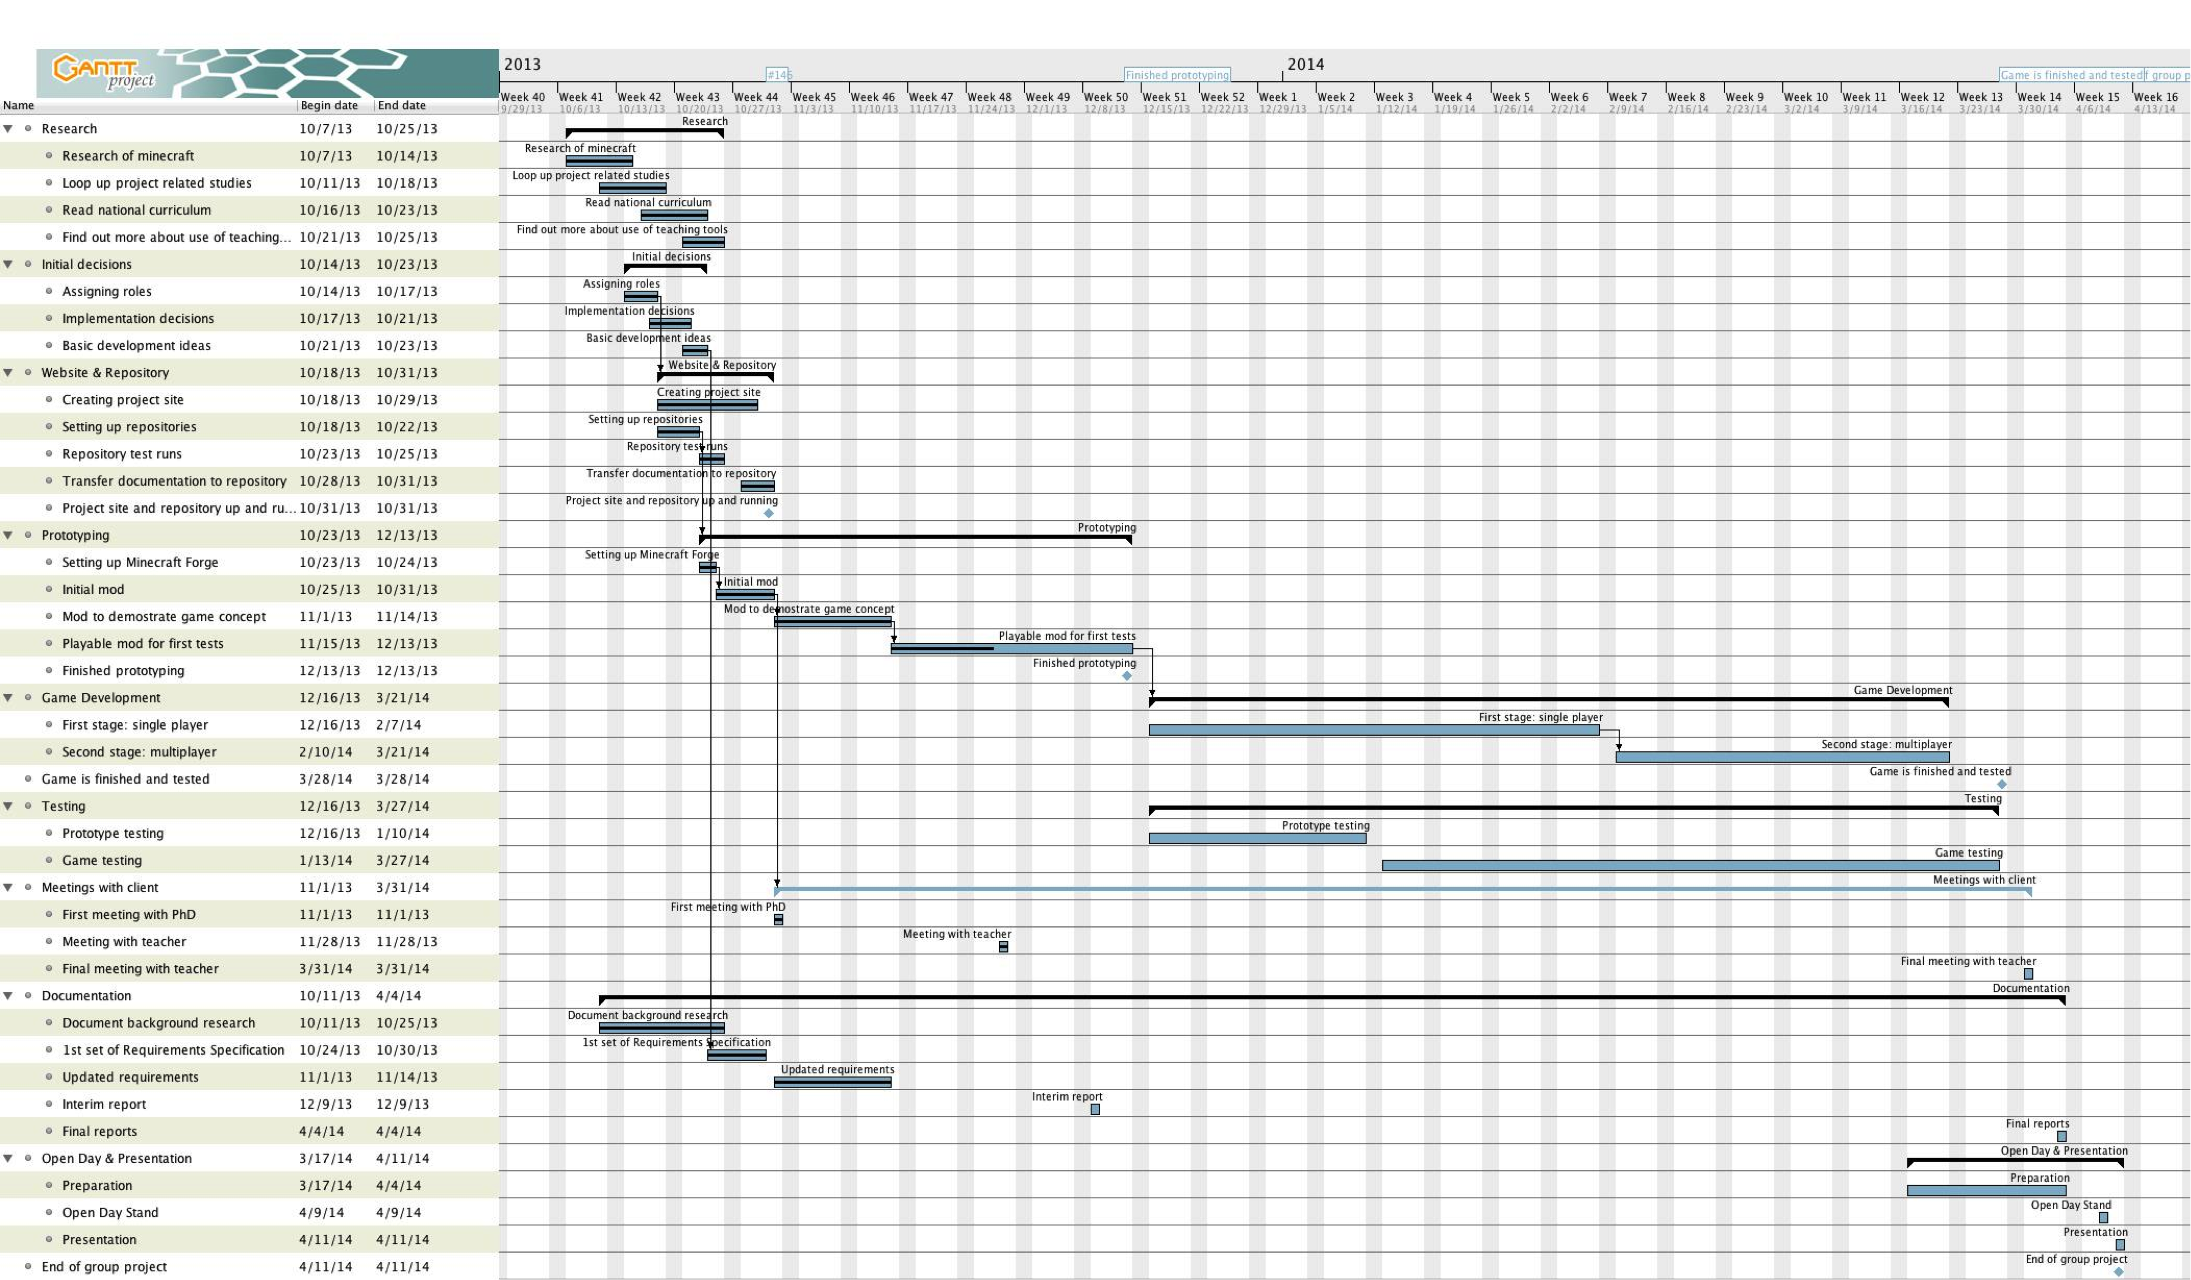
\includegraphics[width=24cm]{interim_gantt_chart}
\end{figure}
\end{landscape}

\bibliography{bibliography}

\end{document}
